%============================================================================%
%
%	DOCUMENT DEFINITION
%
%============================================================================%

%we use article class because we want to fully customize the page and don't use a cv template
\documentclass[10pt,A4]{article}	


%----------------------------------------------------------------------------------------
%	ENCODING
%----------------------------------------------------------------------------------------

% we use utf8 since we want to build from any machine
\usepackage[utf8]{inputenc}		

%----------------------------------------------------------------------------------------
%	LOGIC
%----------------------------------------------------------------------------------------

% provides \isempty test
\usepackage{xstring, xifthen}

%----------------------------------------------------------------------------------------
%	FONT BASICS
%----------------------------------------------------------------------------------------

% some tex-live fonts - choose your own

%\usepackage[defaultsans]{droidsans}
%\usepackage[default]{comfortaa}
%\usepackage{cmbright}
\usepackage[default]{raleway}
%\usepackage{fetamont}
%\usepackage[default]{gillius}
%\usepackage[light,math]{iwona}
%\usepackage[thin]{roboto} 

% set font default
\renewcommand*\familydefault{\sfdefault} 	
\usepackage[T1]{fontenc}

% more font size definitions
\usepackage{moresize}

%----------------------------------------------------------------------------------------
%	FONT AWESOME ICONS
%---------------------------------------------------------------------------------------- 

% include the fontawesome icon set
\usepackage{fontawesome}

% use to vertically center content
% credits to: http://tex.stackexchange.com/questions/7219/how-to-vertically-center-two-images-next-to-each-other
\newcommand{\vcenteredinclude}[1]{\begingroup
\setbox0=\hbox{\includegraphics{#1}}%
\parbox{\wd0}{\box0}\endgroup}

% use to vertically center content
% credits to: http://tex.stackexchange.com/questions/7219/how-to-vertically-center-two-images-next-to-each-other
\newcommand*{\vcenteredhbox}[1]{\begingroup
\setbox0=\hbox{#1}\parbox{\wd0}{\box0}\endgroup}

% icon shortcut
\newcommand{\icon}[3] { 							
	\makebox(#2, #2){\textcolor{maincol}{\csname fa#1\endcsname}}
}	

% icon with text shortcut
\newcommand{\icontext}[4]{ 						
	\vcenteredhbox{\icon{#1}{#2}{#3}}  \hspace{2pt}  \parbox{0.9\mpwidth}{\textcolor{#4}{#3}}
}

% icon with website url
\newcommand{\iconhref}[5]{ 						
    \vcenteredhbox{\icon{#1}{#2}{#5}}  \hspace{2pt} \href{#4}{\textcolor{#5}{#3}}
}

% icon with email link
\newcommand{\iconemail}[5]{ 						
    \vcenteredhbox{\icon{#1}{#2}{#5}}  \hspace{2pt} \href{mailto:#4}{\textcolor{#5}{#3}}
}

\newcommand{\iconegithub}[5]{                         
    \vcenteredhbox{\icon{#1}{#2}{#5}}  \hspace{2pt} \href{#4}{\textcolor{#5}{#3}}
}


%----------------------------------------------------------------------------------------
%	PAGE LAYOUT  DEFINITIONS
%----------------------------------------------------------------------------------------

% page outer frames (debug-only)
% \usepackage{showframe}		

% we use paracol to display breakable two columns
\usepackage{paracol}

% define page styles using geometry
\usepackage[a4paper]{geometry}

% remove all possible margins
\geometry{top=1cm, bottom=1cm, left=1cm, right=1cm}

\usepackage{fancyhdr}
\pagestyle{empty}

% space between header and content
% \setlength{\headheight}{0pt}

% indentation is zero
\setlength{\parindent}{0mm}

%----------------------------------------------------------------------------------------
%	TABLE /ARRAY DEFINITIONS
%---------------------------------------------------------------------------------------- 

% extended aligning of tabular cells
\usepackage{array}

% custom column right-align with fixed width
% use like p{size} but via x{size}
\newcolumntype{x}[1]{%
>{\raggedleft\hspace{0pt}}p{#1}}%


%----------------------------------------------------------------------------------------
%	GRAPHICS DEFINITIONS
%---------------------------------------------------------------------------------------- 

%for header image
\usepackage{graphicx}

% use this for floating figures
% \usepackage{wrapfig}
% \usepackage{float}
% \floatstyle{boxed} 
% \restylefloat{figure}

%for drawing graphics		
\usepackage{tikz}				
\usetikzlibrary{shapes, backgrounds,mindmap, trees}

%----------------------------------------------------------------------------------------
%	Color DEFINITIONS
%---------------------------------------------------------------------------------------- 
\usepackage{transparent}
\usepackage{color}

% primary color
\definecolor{maincol}{RGB}{ 225, 0, 0 }

% accent color, secondary
% \definecolor{accentcol}{RGB}{ 250, 150, 10 }

% dark color
\definecolor{darkcol}{RGB}{ 70, 70, 70 }

% light color
\definecolor{lightcol}{RGB}{245,245,245}


% Package for links, must be the last package used
\usepackage[hidelinks]{hyperref}

% returns minipage width minus two times \fboxsep
% to keep padding included in width calculations
% can also be used for other boxes / environments
\newcommand{\mpwidth}{\linewidth-\fboxsep-\fboxsep}
	


%============================================================================%
%
%	CV COMMANDS
%
%============================================================================%

%----------------------------------------------------------------------------------------
%	 CV LIST
%----------------------------------------------------------------------------------------

% renders a standard latex list but abstracts away the environment definition (begin/end)
\newcommand{\cvlist}[1] {
	\begin{itemize}{#1}\end{itemize}
}

%----------------------------------------------------------------------------------------
%	 CV TEXT
%----------------------------------------------------------------------------------------

% base class to wrap any text based stuff here. Renders like a paragraph.
% Allows complex commands to be passed, too.
% param 1: *any
\newcommand{\cvtext}[1] {
	\begin{tabular*}{1\mpwidth}{p{0.98\mpwidth}}
		\parbox{1\mpwidth}{#1}
	\end{tabular*}
}

%----------------------------------------------------------------------------------------
%	CV SECTION
%----------------------------------------------------------------------------------------

% Renders a a CV section headline with a nice underline in main color.
% param 1: section title
\newcommand{\cvsection}[1] {
	\vspace{14pt}
	\cvtext{
		\textbf{\LARGE{\textcolor{darkcol}{#1}}}\\[-4pt]
		\textcolor{maincol}{ \rule{0.1\textwidth}{2pt} } \\
	}
}

%----------------------------------------------------------------------------------------
%	META SKILL
%----------------------------------------------------------------------------------------

% Renders a progress-bar to indicate a certain skill in percent.
% param 1: name of the skill / tech / etc.
% param 2: level (for example in years)
% param 3: percent, values range from 0 to 1
\newcommand{\cvskill}[3] {
	\begin{tabular*}{1\mpwidth}{p{0.72\mpwidth}  r}
 		\textcolor{black}{\textbf{#1}} & \textcolor{maincol}{#2}\\
	\end{tabular*}%
	
	\hspace{4pt}
	\begin{tikzpicture}[scale=1,rounded corners=2pt,very thin]
		\fill [lightcol] (0,0) rectangle (1\mpwidth, 0.1);
		\fill [maincol] (0,0) rectangle (#3\mpwidth, 0.1);
  	\end{tikzpicture}%
}


%----------------------------------------------------------------------------------------
%	 CV EVENT
%----------------------------------------------------------------------------------------

% Renders a table and a paragraph (cvtext) wrapped in a parbox (to ensure minimum content
% is glued together when a pagebreak appears).
% Additional Information can be passed in text or list form (or other environments).
% the work you did
% param 1: time-frame i.e. Sep 14 - Jan 15 etc.
% param 2:	 event name (job position etc.)
% param 3: Customer, Employer, Industry
% param 4: Short description
% param 5: work done (optional)
% param 6: technologies include (optional)
% param 7: achievements (optional)
\newcommand{\cvevent}[7] {
	
	% we wrap this part in a parbox, so title and description are not separated on a pagebreak
	% if you need more control on page breaks, remove the parbox
    % \parbox{\mpwidth}{
    %     \begin{tabular*}{1\mpwidth}{@{} p{\dimexpr0.59\mpwidth-\tabcolsep} r @{}}
    %         \textcolor{black}{\textbf{#2}} & \colorbox{maincol}{\makebox[0.42\mpwidth]{\textcolor{white}{#1}}} \\
    %         \textcolor{maincol}{\textbf{#3}} & \\
    %     \end{tabular*}\\[8pt]

    %     \ifthenelse{\isempty{#4}}{}{
    %         \cvtext{#4}
    %     }
    % }
    \parbox{\mpwidth}{
      \begin{tabular*}{1\mpwidth}{p{0.59\mpwidth}  r}
          \textcolor{black}{\large{\textbf{#2}}} & \colorbox{white}{\makebox[0.52\mpwidth]{\textcolor{black}{#1}}} \\
          \textcolor{maincol}{\textbf{#3}} & \\
      \end{tabular*}\\[8pt]
    
      \ifthenelse{\isempty{#4}}{}{
          \cvtext{#4}
      }
    }    
	% \parbox{\mpwidth}{
    %   \begin{tabular*}{1\mpwidth}{p{0.59\mpwidth}  r}
    %       \textcolor{black}{\textbf{#2}} & \colorbox{white}{\makebox[0.42\mpwidth]{\textcolor{black}{#1}}} \\
    %       \textcolor{maincol}{\textbf{#3}} & \\
    %   \end{tabular*}\\[8pt]
    
    %   \ifthenelse{\isempty{#4}}{}{
    %       \cvtext{#4}
    %   }
    % } 

	\ifthenelse{\isempty{#5}}{}{
		\vspace{4pt}
		{#5}
	}

	\ifthenelse{\isempty{#6}}{}{
		\vspace{4pt}
		\cvtext{\textbf{Technologies:}}
		{#6}
	}

	\ifthenelse{\isempty{#7}}{}{
		\vspace{4pt}
		\cvtext{\textbf{Achievements:}}
		{#7}
	}
	\vspace{7pt}
}

%----------------------------------------------------------------------------------------
%	 CV META EVENT
%----------------------------------------------------------------------------------------

% Renders a CV event on the sidebar
% param 1: title
% param 2: subtitle (optional)
% param 3: customer, employer, etc,. (optional)
% param 4: info text (optional)
\newcommand{\cvmetaevent}[4] {
	\textcolor{maincol} {\cvtext{\textbf{\begin{flushleft}#1\end{flushleft}}}}

	\ifthenelse{\isempty{#2}}{}{
	\textcolor{darkcol} {\cvtext{\textbf{#2}} }
	}

	\ifthenelse{\isempty{#3}}{}{
		\cvtext{{ \textcolor{darkcol} {#3} }}\\
	}

	\cvtext{#4}\\[14pt]
}

%---------------------------------------------------------------------------------------
%	QR CODE
%----------------------------------------------------------------------------------------

% Renders a qrcode image (centered, relative to the parentwidth)
% param 1: percent width, from 0 to 1
\newcommand{\cvqrcode}[1] {
	\begin{center}
		
\includegraphics[width={#1}\mpwidth]{qrcode}
	\end{center}
}


%============================================================================%

%%
%
%	DOCUMENT CONTENT
%
%
%
%============================================================================%
\begin{document}
\columnratio{0.31}
\setlength{\columnsep}{2.2em
}\setlength{\columnseprule}{4pt}
\colseprulecolor{lightcol}
\begin{paracol}{2}
\begin{leftcolumn}
%---------------------------------------------------------------------------------------
%	META IMAGE + info
%----------------------------------------------------------------------------------------
%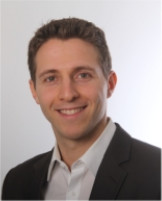
\includegraphics[width=\linewidth]{untitled.jpg}	%trimming relative to image size



\vfill\null
\cvsection{Contact}
	
\icontext{MapMarker}{12}{Puy de Merland\\24110 St Astier, France}{black}\\[6pt]
\icontext{MobilePhone}{12}{+33 6 75 10 87 20}{black}\\[6pt]
\iconemail{Envelope}{12}{ha.lagrange9000@gmail.com}{ha.lagrange9000@gmail.com}{black}\\[6pt]
\iconegithub{Github}{12}{https://github.com/Dedalum}{https://github.com/Dedalum}{black}\\


%---------------------------------------------------------------------------------------
%	META SKILLS
%----------------------------------------------------------------------------------------
\cvsection{Technical skills}

\cvskill{Python} {5+ yrs} {0.8} \\[-2pt]

\cvskill{Golang} {2+ yrs} {0.6} \\[-3pt]

\cvskill{SQL} {5+ yrs} {0.7} \\

\cvskill{Linux, Bash, git} {5+ yrs} {1} \\[-2pt]

\cvskill{Ansible, Jenkins} {3+ yrs} {0.5} \\[-3pt]

\cvskill{AWS/GCP, Kubernetes} {2+ yrs} {0.4} \\[-3pt]

\cvskill{Elasticsearch, InfluxDB \& Grafana} {2+ yrs} {0.4} \\[-3pt]

\cvskill{HTML/CSS (Tailwind), JS, Nuxt/VueJS} {1+ yrs} {0.3} \\[-4pt]

\vfill\null
\cvsection{Other skills}

\cvskill{Agile methods: Scrum \& Kanban} {5+ yrs} {1} \\[-2pt]

\cvskill{Product development \& management} {3+ yrs} {0.65} \\[-2pt]

\cvskill{Cross-team communication} {5+ yrs} {1} \\

\cvskill{Customer support} {4+ yrs} {1} \\

\cvskill{SEO \& Web marketing} {<1 yr} {0.2} \\[-3pt]

\vfill\null
\cvsection{Languages}
{\cvlist{
    \item French: native speaker
    \item English: full proficiency
    \item German, Swedish, Spanish: basic level
}}


%---------------------------------------------------------------------------------------
%	EDUCATION
%----------------------------------------------------------------------------------------
\cvsection{Education}

\cvmetaevent
{2011 - 2016}
{Master degree, IT \& CS}
{Université de Technologie de Troyes - Troyes, France}
{IT \& CS, specializing in Information Security: mathematics, networking,
Computer Science, relational DB, image processing, cryptography,
information security (policies and management of information)}

\cvmetaevent
{Fall 2014}
{Exchange }
{University of Waterloo - Waterloo, Canada}
{Faculty of mathematics, computer science program: computer \& information security, CS, graph theory}

% -------
% Extra
% -------

\cvsection{Interests}
{\cvlist{
    \item Crypto/blockchain technologies and markets
    \item Business \& marketing \& startups
    \item History \& international relations, infosec \& osint
    \item Language learning, cultures, \\books
    \item Beer brewing, hiking
}}

%---------------------------------------------------------------------------------------
%	CERTIFICATION
%----------------------------------------------------------------------------------------
% \newpage
% \cvsection{CERTIFICATIONS}

% \cvmetaevent
% {LPIC 1 - Linux administrator}
% {}
% {}
% {Certificate issued by the Linux Professional Institute to prove abilities in Linux administration}


\end{leftcolumn}
\begin{rightcolumn}
%---------------------------------------------------------------------------------------
%	TITLE  HEADER
%----------------------------------------------------------------------------------------
\fcolorbox{white}{white}{\begin{minipage}[c][3.5cm][c]{1\mpwidth}
	\begin {center}
		\HUGE{ \textbf{ \textcolor{black}{ Hugues Lagrange } } } \\[-20pt]
		\textcolor{black}{ \rule{0.1\textwidth}{1.25pt} } \\[4pt]
		\large{ \textcolor{black} {Developer/devops} }
	\end {center}
\end{minipage}} \\[1pt]
\vspace{-12pt}

%---------------------------------------------------------------------------------------
%	PROFILE
%----------------------------------------------------------------------------------------
\vfill\null
\cvsection{PROFILE}

\cvtext{Looking for challenges, exciting products and good team spirit. Flexible and adaptive tech person diving into business and marketing with specific experience in Python and Golang in the fintech industry. Devops and automation mindset, problem solver and open-minded.
}

%---------------------------------------------------------------------------------------
%	WORK EXPERIENCE
%----------------------------------------------------------------------------------------
\vfill\null
\cvsection{WORK EXPERIENCE \& PROJECTS}

\cvevent
    {Feb 23 - May 23, 4 mo}
    {Professional project: software \& product development}
    {PDF Toolkit API - Remote, France}
    {Building a SaaS company from scratch providing an API to generate various types of PDF documents including receipts, reports, resumes in a team of 2.}
    {\cvlist{    
        \item Building a production-ready API using Python and FastAPI following TDD, a developer's documentation with VitePress and OpenAPI and a blog with VitePress
        \item Deployment and maintenance of the production environment with Github Actions (CI), Ansible, Traefik
        \item Design and maintenance of an PostgreSQL database
        \item InfluxDB \& Grafana for metrics
        \item Setting up an SEO \& web marketing strategy, business development, analytics with the help of AI (ChatGPT/OpenAI API)
    }}
    {}
    {}

\cvevent
	{Apr 20 - Aug 23, 3 yr 5 mo}
	{Software developer - Python}
	{Linxo Group - Remote/Aix-en-Provence, France}
	{Linxo is a French fintech startup aggregating banking data for individuals and offering services of accounting and business finance for businesses.\\
    I was part of the team responsible for aggregating the banking data and handling its pipelines and its pre-analysis in a GDPR compliant \& ISO 27001 certificated environment.}
    {\cvlist{
        \item Design and implementation of features and business logic for banking and financial data gathering
        \item Within an 8 people company-wide cross-team, design \& implementation of the "wealth" service gathering and analyzing financial investments \& portfolios data for businesses and customers
        \item Building a PoC "crypto" service gathering crypto-currencies investments \& portfolios and providing analysis for our customers
        \item Meetings \& monthly exchanges with French and foreign banks for issues solving and feature developments
        \item Handling level 3 customer support, including business customers and simple users
    }}
    {\cvlist{
      \item Python, PostgreSQL, occasional Java/Go
      \item Jenkins CI, ELK stack for logging, Grafana metrics (Postgres, Influxdb), Bash
    }}
    {}

% \vfill\null
\cvevent
	{May 17 - Aug 18, 1 yr 4 mo}
    {Software developer - Golang \& Python}
    {Snuk - Berlin, Germany}
    {Early-stage startup building an IoT infrastructure platform for smart buildings.}
    {\cvlist{
        \item Design of distributed systems, implementation and installation of on-premise IoT infrastructures and cloud architectures
        \item Direct product development with the customers and remote \& on-site support with the factories management and workers
    }}
    {\cvlist{
        \item Golang \& Python development, Bash
        \item GCP, Docker, Hashicorp stack, Ansible, Linux
        \item TIGK stack (Grafana, Telegraf, Influxdb, Kapacitor)
        \item Postgres, MongoDB
        \item IoT, BLE, MQTT, Mosquitto, Raspberry Pi
	}}
    {}

% \vfill\null
\cvevent
    {Mar 16 - Sep 16, 6 mo}
    {IT security/admin intern}
    {Freespee AB - Uppsala, Sweden}
    {Freespee is a real time conversation cloud for marketers. AWS, ELK stack \& Redis, Ansible, OpenVPN server, Linux, Bash \& Python scripting.}
    % I worked as an intern in the engineering team, in Uppsala, Sweden, performing system administration tasks with a focus on information security. Along my different projects were}
    % {\cvlist{
    %     \item Deploying an ELK stack for central log management with a Redis buffer in an AWS VPC (25 VMs)
    %     \item Preparing an office firewall based on Debian (iptables scripts, Suricata IDS, OpenVPN bridge, VLANs, DHCP and local DNS)
    %     \item Installing an OpenVPN server for a secure remote access to the AWS VPC
    %     \item Research and setup of a ”chatops” solution using Slack and Errbot, Jenkins, Ansible and Docker 
    % }}
	{}
    {}
	{}

% \vfill\null
\cvevent
    {Feb 15 - Jul 15, 6 mo}
    {System administrator}
    {Jymeo - Nantes, France}
    {JYMEO is an internet/marketing start-up. OVH cloud, ELK stack, Ansible, OpenVPN server, Linux, Bash \& Python scripting.
    }
     % We followed the Scrum method. I deployed and worked on the ELK suite for analyzing server logs, deployed OpenVPN servers and backup scripts, firewalls (iptables, fail2ban, NAXSI), secured Wordpress websites.}
    % {\cvlist{
    %     \item Setting up new servers (Virtual machines running Debian 8, with providers OVH/RunAbove) with web-servers (Nginx, Apache)
    %     \item Level 3 support
    % }}
    {}
    {}
    {}

% hotfixes to create fake-space to ensure the whole height is used
\mbox{}
\vfill
\mbox{}
\vfill
\mbox{}
\vfill
\mbox{}
\end{rightcolumn}
\end{paracol}
\end{document}

